\section{Experiments of planning grasps for non-familiar objects}
\label{cha3:sec5}


\begin{table*}
\renewcommand{\arraystretch}{1.5}
\hspace{-2cm}
    \begin{tabular}
    { |>{\centering\arraybackslash}p{4cm}  | c | c | c | c |}
    \hline
    Approach and object & Force-Closure Grasp Found &  Mean of Computation Time($msec$) & Variance ($msec$)   \\ \hline
    Pre-trained grasp GMM for the novel object       & 98.1\%  & 13.8    & 0.015 \\ \hline
    Combined grasp GMM for novel object             & 92.1\%  & 21.9    & 0.011 \\ \hline
    Combined grasp GMM for spray flask              & 91.0\%  & 16.0    & 0.004 \\ \hline
    Combined grasp GMM for bedside table            & 82.2\%  & 21.1    & 0.006 \\ \hline
    \end{tabular}
\caption{Success rate and computation time of different methods and objects}
\label{tab:result}
\end{table*}

\begin{table*}
\renewcommand{\arraystretch}{1.5}
\hspace{-2cm}
    \begin{tabular}
    { | c | c | c |>{\centering\arraybackslash}p{3cm} |>{\centering\arraybackslash}p{3cm}|}
    \hline
    Shape primitives& Object & Size($cm$) & Number of training data & Number of Gaussians in GMM   \\ \hline
    Sphere 1        & Novel object (Fig.~\ref{fig:object})  & radius 7              & 12096    & 60 \\ \hline
    Cylinder 1      & Novel object (Fig.~\ref{fig:object})  & height 15 and radius 4& 15608    & 60 \\ \hline
    Box 1 & Spray flask (Fig.~\ref{fig:spr})        & $6\times9.5\times8$       & 9256    & 40 \\ \hline
    Box 2 & Spray flask (Fig.~\ref{fig:spr})        & $4\times11\times4.5$      & 7544    & 40 \\ \hline
    Box 3 & Spray flask (Fig.~\ref{fig:spr})        & $2.5\times4\times7$       & 3400    & 30 \\ \hline
    Box 4 & Bedside table (Fig.~\ref{fig:bedside})  & $52.5\times3\times52.5$   & 8668    & 20 \\ \hline
    Box 5 & Bedside table (Fig.~\ref{fig:bedside})  & $2.8\times57.6\times2.7$  & 4392    & 20 \\ \hline
    \end{tabular}
\caption{Shape primitives used in experiments}
\label{tab:primitive}
\end{table*}

We test our approach initially on a novel object that is a combination of a sphere and a cylinder (Figure.~\ref{fig:object}(a) and Table~\ref{tab:primitive}). We choose to use the Barrett hand for the implementation as it is available in our lab. As explained above, the grasp of the Barrett hand is formulated as the combination of the hand position ($h$), orientation($o$) and finger joint angles($\theta$).  The grasp GMMs of the sphere and cylinder are pre-trained with randomly generated stable grasps from the simulator GraspIt!.

We compare this new approach with the previous approach that directly trained a grasp GMM for the whole object, by generating grasps for the object from 1000 starting points. Figure.~\ref{fig_result} shows a few resulting grasps. As shown in the Table~\ref{tab:result}, the success rate and the computation time of the new approach is of the same scale as the previous approach. The computation time is computed by Matlab on a machine with 4GB RAM.
/textcolor{red}{CPU speed in GHz probably relevant here too}

Further, we train 5 different boxes as our primitives (Table~\ref{tab:primitive}) and use them to approximate two daily life objects: a spray flask and a bedside table. The spray flask is approximated as the combination of box 1, 2 and 3 (Figure.~\ref{fig:spr}) and the bedside table is approximated as the combination of box 4 and 5 (three copies of box 4 as the surfaces and 4 copies of box 5 as the legs). The result is shown in Table~\ref{tab:result}. A few initial hand postures and their resulting grasps are shown in Fig~\ref{fig:spr_result} and~\ref{fig:result:bedside}.

%\vspace{-0.2in}
\begin{figure}
%\vspace{-0.3cm}
\centering
    \subfloat[\scriptsize{Initial pose 1}]  {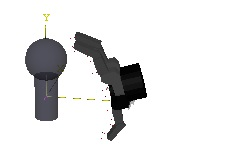
\includegraphics[width=1.05in]{./fig_cha3/8_i.jpg}}
    %\hspace{-0.01in}
    \subfloat[\scriptsize{Initial pose 2}] {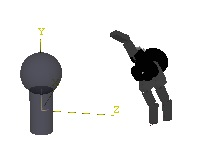
\includegraphics[width=1.05in]{./fig_cha3/1_i.jpg}}
    %\hspace{0.01in}
    \subfloat[\scriptsize{Initial pose 3}] {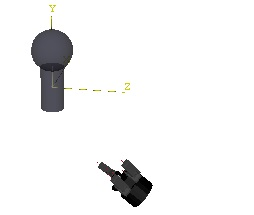
\includegraphics[width=1.05in]{./fig_cha3/5_i.jpg}}
    %\vspace{0.05in}

    \subfloat[\scriptsize{Final grasp 1}] {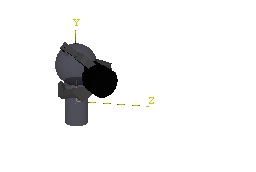
\includegraphics[width=1.05in]{./fig_cha3/8_f.jpg}}
    \hspace{0.005in}
    \subfloat[\scriptsize{Final grasp 2}] {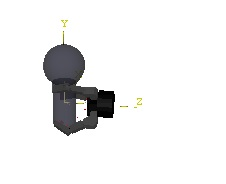
\includegraphics[width=1.05in]{./fig_cha3/1_f.jpg}}
    \hspace{0.005in}
    \subfloat[\scriptsize{Final grasp 3}] {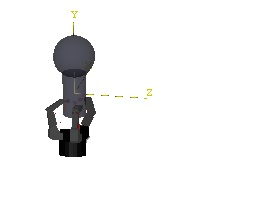
\includegraphics[width=1.05in]{./fig_cha3/5_f.jpg}}

    \subfloat[\scriptsize{3D projections}] {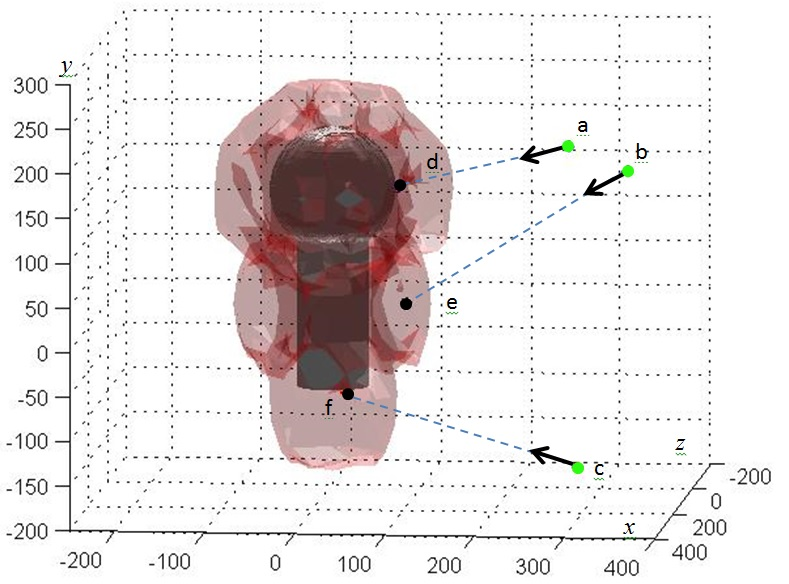
\includegraphics[width=1.8in]{./fig_cha3/object_cylball_i_f_arrow.jpg}}
    \hspace{0.005in}
    \subfloat[\scriptsize{2D contour projections}] {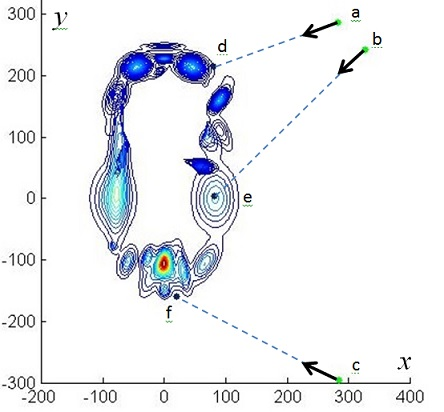
\includegraphics[width=1.4in]{./fig_cha3/contour_Z_cylball_i_f_arrow2.jpg}}

\caption{\scriptsize{Examples of Barrett hand grasping of a novel object. (a-d) Initial hand postures and final grasps. (g) A 3D illustration of the projection between the initial hand postures and the final grasps. (h) a 2D illustration of the interaction of GMM at $z$ = 0.}}

%\vspace{-0.2cm}
\label{fig_result}
\end{figure}

\begin{figure}
\centering
    \subfloat[\scriptsize{}]  {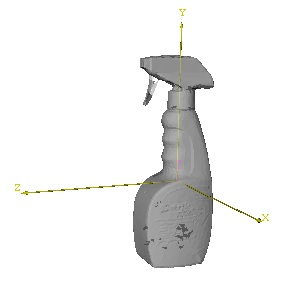
\includegraphics[width=5cm]{./fig_cha3/spr.jpg}}
    \hspace{1cm}
    \subfloat[\scriptsize{}] {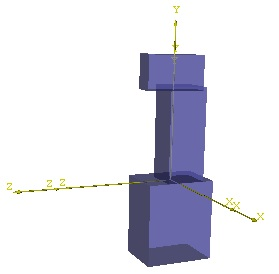
\includegraphics[width=5cm]{./fig_cha3/box123.jpg}}
%    \hspace{0.01in}
\caption{\scriptsize{(a) A spray flask. (b) A spray flask approximated by 3 boxes.}}
\label{fig:spr}
\end{figure}



\begin{figure}
\centering
    \subfloat[\scriptsize{Initial pose 1}]  {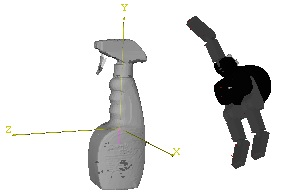
\includegraphics[height= 4cm]{./fig_cha3/spr_3_i.jpg}}
    \hspace{1cm}
    \subfloat[\scriptsize{Initial pose 2}] {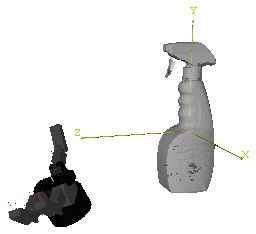
\includegraphics[height= 4cm]{./fig_cha3/spr_4_i.jpg}}
    \hspace{1cm}
    \subfloat[\scriptsize{Initial pose 3}] {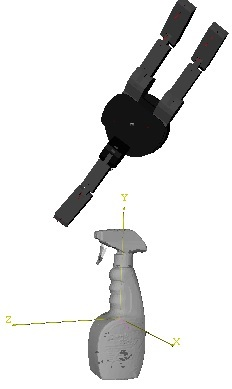
\includegraphics[height= 4cm]{./fig_cha3/spr_6_i.jpg}}

    %\vspace{0.05in}
    \subfloat[\scriptsize{Final grasp 1}] {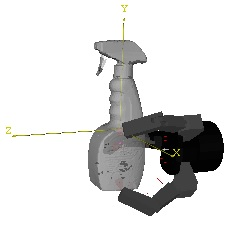
\includegraphics[width=4cm]{./fig_cha3/spr_3_f.jpg}}
    \hspace{1cm}
    \subfloat[\scriptsize{Final grasp 2}] {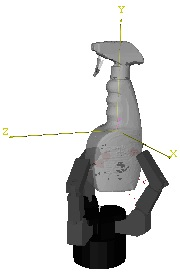
\includegraphics[height=4cm]{./fig_cha3/spr_4_f.jpg}}
    \hspace{1cm}
    \subfloat[\scriptsize{Final grasp 3}] {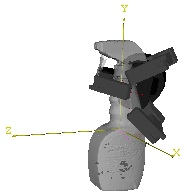
\includegraphics[width=4cm]{./fig_cha3/spr_6_f.jpg}}

\caption{\scriptsize{Examples of Barrett hand grasping of a spray flask. }}
%\vspace{-0.8cm}
\label{fig:spr_result}
\end{figure}


\begin{figure}
\centering
    \subfloat[\scriptsize{}]  {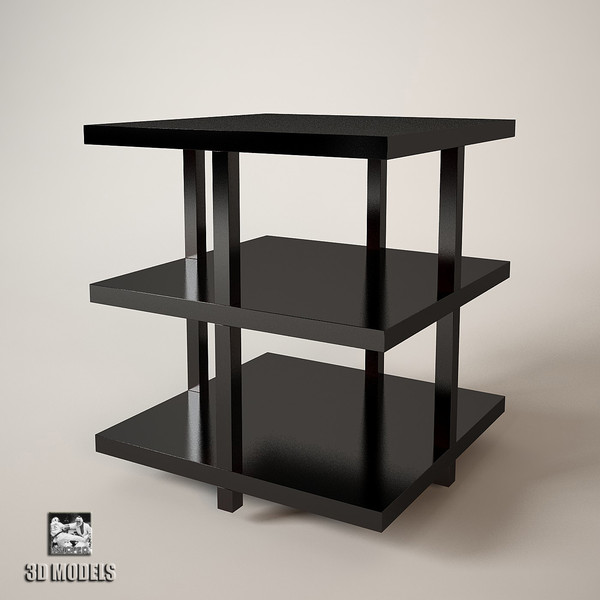
\includegraphics[width=5cm]{./fig_cha3/bedside.jpg}}
    \hspace{0.07in}
    \subfloat[\scriptsize{}] {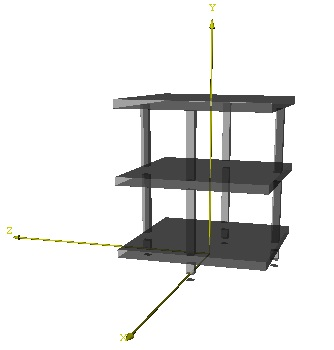
\includegraphics[width=5cm]{./fig_cha3/bedside_box.jpg}}
%    \hspace{0.01in}
\caption{\scriptsize{(a) A bedside table. (b) A bedside table approximated by 7 boxes.}}
\label{fig:bedside}
\end{figure}

\begin{figure}
\centering
    \subfloat[\scriptsize{Initial pose 1}]  {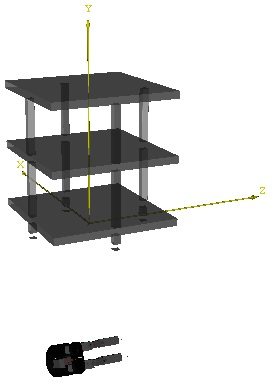
\includegraphics[width=4cm]{./fig_cha3/bed_6_i.jpg}}
    \hspace{0.2cm}
    \subfloat[\scriptsize{Initial pose 2}] {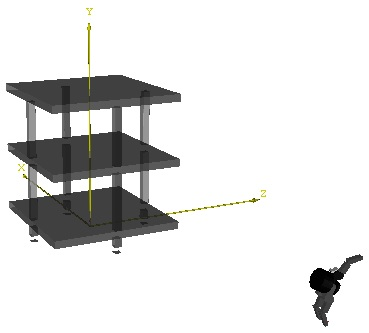
\includegraphics[width=4cm]{./fig_cha3/bed_3_i.jpg}}
    \hspace{0.7cm}
    \subfloat[\scriptsize{Initial pose 3}] {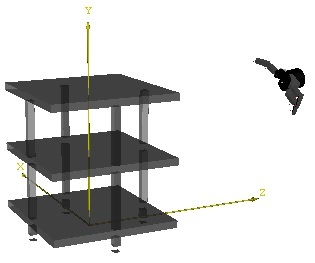
\includegraphics[width=4cm]{./fig_cha3/bed_5_i.jpg}}
    %\vspace{0.05in}

    \subfloat[\scriptsize{Final grasp 1}] {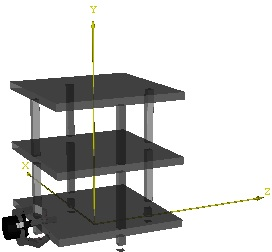
\includegraphics[width=4cm]{./fig_cha3/bed_6_f.jpg}}
    \hspace{0.005in}
    \subfloat[\scriptsize{Final grasp 2}] {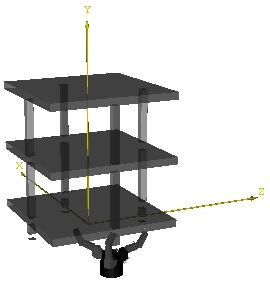
\includegraphics[width=4cm]{./fig_cha3/bed_3_f.jpg}}
    \hspace{0.005in}
    \subfloat[\scriptsize{Final grasp 3}] {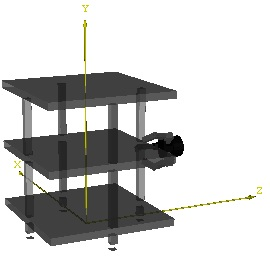
\includegraphics[width=4cm]{./fig_cha3/bed_5_f.jpg}}


\caption{\scriptsize{Examples of Barrett hand grasping of a complex shape bedside table (a-d) Initial hand postures and final grasps. }}
\label{fig:result:bedside}
\end{figure}


%$\bullet$ TODO: grasp density can be used to find grasps by task (Detry)
%$\bullet$ TODO: can not find grasps over different parts
%$\bullet$ TODO: interpolate primitives?
%$\bullet$ TODO: human spend more time on new object
%$\bullet$ TODO: take volume of robot hand into account
%In implementation we found the success rate depends on how well we can approximate the novel object with known shape primitives, and hence the choice of the shape primitives is important.Future work will focus on studying how to interpolate the grasp GMM for different shape primitives, to allow the novel objects to be approximated more precisely.

